\section{Simulador}
\ \\ Al iniciar la aplicacion se mostrará un menu principal, acontinuacion explicaremos cada uno de ellos:\\

\begin{figure}[htbp]
\begin{center}
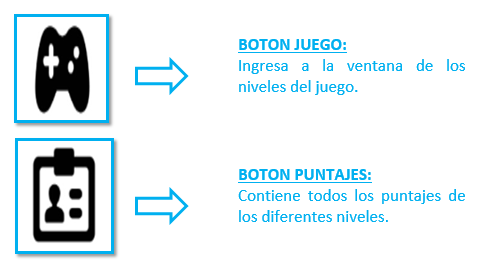
\includegraphics[width=.70\textwidth]{./imagenes/controles1.png}
\caption{Menu Principal 1}
\label{MenuPrincipal}
\end{center}
\textbf{Boton de Juego}: Este bóton es con el que se inicia a un nuevo juego, al presionar este bóton se le pedira al usuario el nivel de juego que quisisera empezar a jugar.\\
\textbf{Boton Puntajes}: Este bóton indica los records que hay por cada nivel, el record de cada jugador se graba una vez que el jugador haya ganado el juego.
\end{figure}

\begin{figure}[htbp]
\begin{center}
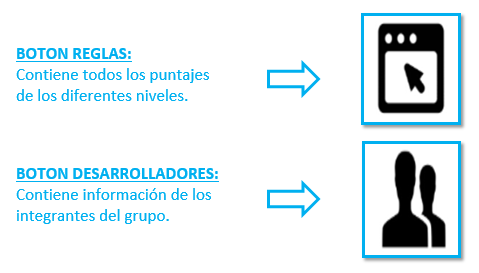
\includegraphics[width=.70\textwidth]{./imagenes/C.png}
\caption{Menu Principal 2l}
\label{MenuPrincipal}
\end{center}
\textbf{Boton Reglas}: Se indica las reglas con las que se juega, una vez empezado el juego.\\
\textbf{Boton Desarrolladores}: Presionando este boton se indican los nombres y datos adicionales de los creadores de la aplicación Buscaminas.\\
\end{figure}
\ \\ \ \\ \ \\ \ \\

\begin{figure}[htbp]
\begin{center}
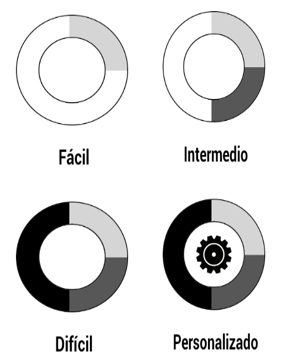
\includegraphics[width=.70\textwidth]{./imagenes/Niveles.png}
\caption{Nivel de Dificultad}
\label{Nivel de Dificultad}
\end{center}
Al presionar el bóton de Juego se le pedira al usuario escoger el nivel al que quiera empezar a jugar. Se tiene 4 niveles:
\\ \textbf{Facill} : 8 x 8  y 10 minas.
\\ \textbf{Intermedio}: 10 x 10 y 15 minas.
\\ \textbf{Dificil}: 12 x 12 y 20 minas.
\\En caso de Presionar el nivel de Dificultad: \textbf{Personalizado}: Se le pedira al jugador que eliga con que cantidad 
\\de filas, columnas y minas desea empezar a jugar.  
\end{figure} 
\ \\ \ \\ \ \\ \ \\

\begin{figure}[htbp]
\begin{center}
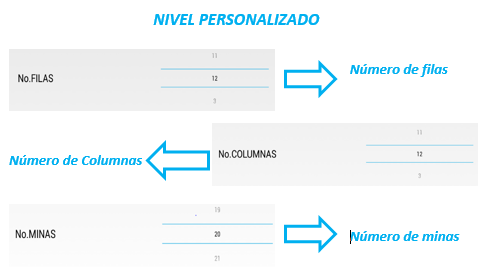
\includegraphics[width=.70\textwidth]{./imagenes/Personalizado.png}
\caption{Personalizado}
\label{Personalizado}
\end{center}
En cuanto el usuario escogio el nivel personalizado, se le pide que escoga la cantidad de filas, columnas y minas 
\\con las que el jugador quiera empezar a jugar, cabe recalcar que la cantidad de minas depende de las filas y columnas
\\con las que quiera jugar, es decir la cantidad de minas no puede ser mayor al número de celdas que se encuentren en
\\el juego. 
\end{figure} 
\ \\ \ \\ \ \\ \ \\

\begin{figure}[htbp]
\begin{center}
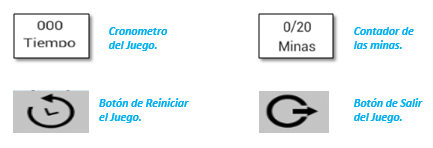
\includegraphics[width=.70\textwidth]{./imagenes/botonesR.png}
\caption{Botones en Ventana de juego}
\label{Juego}
\end{center}
En la Ventana de Juego tenemos las siguientes caracteristicas:
\\Cronometro del Juego: Indica el Tiempo que se lleva jugando la partida, cabe indicar que este tiempo solo marca en \\segundos
\\Contador de las minas: Indica la cantidad de banderas que debemos de colocar en la que suponemos que se encuentra
\\una mina, esto es una ayuda para el jugador.
\\Botón de reiniciar el juego: Presionando este bóton se reinicia el juego, indicamos que no será el mismo juego que
\\anteriormente lo jugaba.
\\Botón de Salir del Juego: Presionandolo saldremos del juego, es decir la aplicacion se cerrará.
\end{figure} 
\ \\ \ \\
\begin{figure}[htbp]
\begin{center}
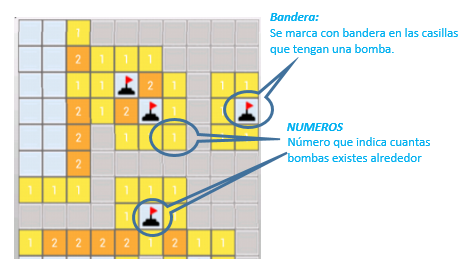
\includegraphics[width=.70\textwidth]{./imagenes/Tabla1.png}
\caption{Juego}
\label{Juego}
\end{center}
Para descubrir una celda se la presiona, en el cual se descubre si es o no una mina, en caso de que no sea mina
\\ al descubrir se indicara la cantidad de minas que esa celda tenga alrededor de ella.
\\Para marcar la celda se debe de mantener presionada alrededor de 2 segundos, hasta que la celda tome la figura
\\de una bandera de color rojo.
\end{figure} 
\ \\ \ \\
\begin{figure}[htbp]
\begin{center}
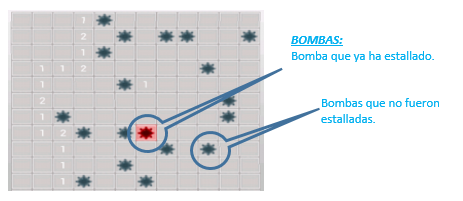
\includegraphics[width=.70\textwidth]{./imagenes/Tabla2.png}
\caption{Juego Perdido}
\label{Juego Perdido}
\end{center}
Una vez que se descubre a una mina, el jugador pierde la partida. En el tablero se resalta la mina que exploto
\\y se descubren todas las minas del tablero.
\end{figure} 